\section{Etudes des vues fonctionnelles}

Pendant le premier moins de l’étude de l’existant, j’ai aussi réalisé les codes de l’édition dans un projet d’ezb de la version d’Ophir. Mais après montré le page d’édition à ec, j’étais informé qu’il n’était pas suffisant pour l’utilisation prévue. De plus, la plate-forme était attendu à reconnaître des différents types d’utilisateurs \footnote{Des enseignants et des élèves au principe} et  faire une distinction entre eux. Cependant, il n’y avait pas un cahier de charge défini des fonctions nécessaires d’ezb. 

Après plusieurs réunions avec ec, tls et des autres enseignants-chercheurs participant dans le développement d’ezb, on a réussi de définir une liste fonctionnelle qui bien indique des fonctions principales et des fonctions supplémentaires :

\begin{enumerate}
    \item La gestion d'utilisateurs 
    \begin{itemize}
        \item Accès permettant d’entrer la plate-forme avec le compte de l’école
        \item Reconnaissance d’identités entre des enseignants et des élèves
        \item Trois niveau de droits autorisés aux différent types d’utilisateurs selon leur identité
            \begin{itemize}
                \item Utilisateur Root
                \item Utilisateur Supérieur
                \item Utilisateur Ordinaire
            \end{itemize}
        \item Des messageries distribuées à chaque utilisateur pour des annonces des systèmes
    \end{itemize}
    \item La gestion de livres
    \begin{itemize}
        \item Création de livre à partir des fichiers en multi-format
        \item Définition de droits d’autorisation 
        \item Des autres manipulations nécessaires
        \item Téléchargement de livre en multi-format 
    \end{itemize} 
    \item La gestion de projets
    \begin{itemize}
        \item Création d'un projet à partir d'un projet existant ou d'un livre
        \item Définition de plusieurs finalités comprenant une qui permet de couper le livre dans plusieurs morceaux et les distribuer aux sous-groupes d’élèves
        \item Contribution collaboration
        \item Manipulations de layers \footnote{Des layers sont des couches sur lesquelles on travaille}
        \item Editions synchronisées dans un layers
        \item Copie d'un projet en choisissant des layers disponibles
        \item Définition d'autorisation à un groupe mais aussi des autres invités
    \end{itemize}
    \item La gestion de groupes
    \begin{itemize}
        \item Création d'un groupe et définir un manager
        \item Modification du groupe
    \end{itemize}   
\end{enumerate}

Pour préciser des fonctions autorisées aux différents type d’utilisateurs, j’ai fait un tableau de définition :
\begin{figure}[H]
\centering
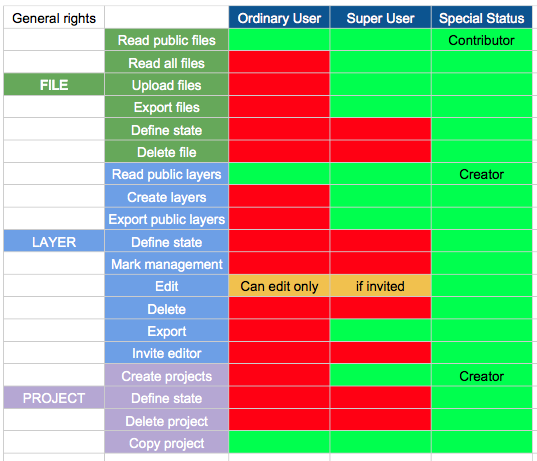
\includegraphics[width=\textwidth]{droits1}
\caption{Droits générals}
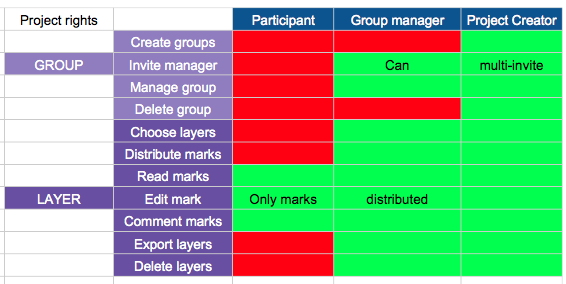
\includegraphics[width=\textwidth]{droits2}
\caption{Droits de projets}
\end{figure}
\begin{figure}[H]
\centering
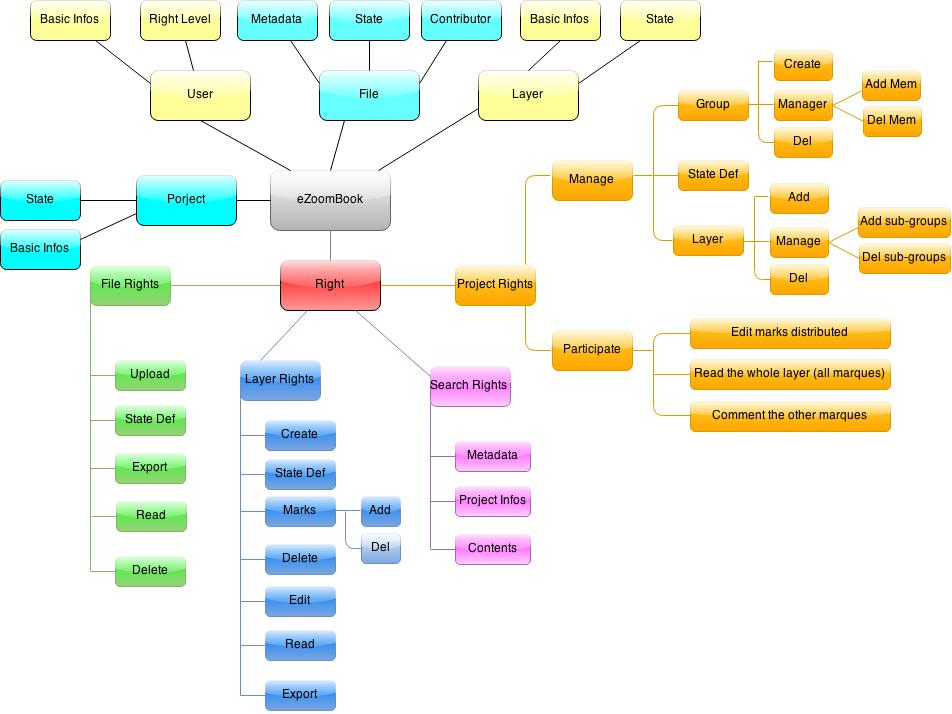
\includegraphics[width=\textwidth]{fonctions}
\caption{Fonctions de projets}
\end{figure}